\documentclass[letterpaper,11pt]{article}

\usepackage[spanish,english]{babel}
\usepackage[top=2cm,bottom=2cm,right=2cm,left=2cm]{geometry}
\usepackage{circuitikz}
\usepackage{amssymb}
\usepackage{amsmath}
\usepackage{amsthm}
\usepackage{mathrsfs}
\usepackage{empheq}
\usepackage{emptypage}
\usepackage{mdframed}
\usepackage{booktabs}
\usepackage{lipsum}
\usepackage{graphicx}
\usepackage{color}
\usepackage{psfrag}
\usepackage{pgfplots}
\usepackage{bm}
\usepackage{multicol}
\usepackage{wrapfig}
\usepackage{float}
\usepackage{fancyhdr}
\usepackage{wrapfig}
\usepackage{multirow}
\usepackage{csquotes}
\usepackage{parskip}
\usepackage{cancel}
\usepackage{listing}
\usepackage{tikz}
\usepackage{verbatim}
\usepackage{subcaption}
\usepackage{enumitem}
\usepackage{xcolor}
\usepackage{xfrac}
\usepackage{hyperref}

\graphicspath{{fig/}}
%\addbibresource{biblio.bib}
\usepgfplotslibrary{colorbrewer}
\pgfplotsset{width=8cm,compat=1.9}
\definecolor{negro}{RGB}{0,0,0}
\definecolor{azul}{RGB}{0,0,255}
\definecolor{verde}{RGB}{0,255,0}
\definecolor{cian}{RGB}{0,255,255}
\definecolor{rojo}{RGB}{255,0,0}
\definecolor{magenta}{RGB}{255,0,255}
\definecolor{amarillo}{RGB}{255,255,0}
\definecolor{blanco}{RGB}{255,255,255}

\definecolor{limegreen}{cmyk}{0.75,0,1,0}
\definecolor{orange}{cmyk}{0,0.8,0.95,0}
\definecolor{purple}{cmyk}{0.75,1,0,0}
\begin{document}
\begin{center}
    \vspace{12mm}

    \LARGE{\textit{Ecuación de Rayleigh con ruido estocástico.}}
    \vspace{3mm}
    
    \textit{\large{Fajardo Fernando, Ospina Juan P.}}
    \vspace{1mm}
            
    \normalsize{12 de Octubre, 2026}
    \vspace{10mm}
\end{center}

\vspace{35pt}

\Large


\begin{center}

    \textbf{Resumen}
    
        Se resuelve la ecuación diferencial no lineal del oscilador de Rayleigh con ruido estocástico $\xi(t)$ mediante reducción de orden ---$\dot{x} = v$--- y la posterior discretización del sistema para $n$ paso utilizando el método de  Euler–Maruyama y Heun; posteriormente, se compararon soluciones para tres configuraciones de posición y velocidad inicial presentes en la carpeta del proyecto ubicados en $../\text{results}/\text{Temp}$ con las configuraciones: (1,0),(0,1),(-1,0)) y cuatro valores de $\sigma$ 0, 0.2, 0.5 y 1.
    
    \vspace{10pt}
     
        \textbf{Palabras clave} --- \textit{Oscilador, Rayleigh, Ruido, Estocástico, Aproximación}
    
    \vspace{25pt}
     
\end{center}

\begin{multicols}{2}

\section*{Introducción}

    Se tiene la ecuación diferencial de Rayleigh con ruido:

    \begin{align*}
        \ddot{x} + \epsilon \Bigg(\frac{\dot{x}^2}{3} - 1 \Bigg)\dot{x} + x = \sigma \xi(t)
    \end{align*}

    La cuál es una ecuación \textit{no} lineal caracterizada por el término correspondiente a la primer derivada temporal conocida como \textit{amortiguamiento no lineal} dado que cuando $\dot{x}<3$, el sistema entra en resonancia, se le agrega energía; mientras que cuando $\dot{x}>3$, se disipa energía y el sistema frena; además, se tiene el parámetro $\epsilon$ el cual multiplica los efectos del amortiguamiento y para el caso $\epsilon \longrightarrow 0$, el sistema se aproxima a un oscilador armónico lineal.

    Por otra parte, se tiene el término $\sigma \xi(t)$ que representa un fuente de ruido o forzamiento externo al sistema el cual habitualmente es modelado como ruido blanco gaussiano y $\sigma$ determina la intensidad de dicho ruido.

    Inclusive, se logra obtener el caso determinista cuando no hay ruido externo ---$\sigma = 0$---, llegando a la ecuación de Rayleigh «pura» donde debido al balance entre la ganancia de energía a bajas velocidades y la disipación a altas velocidades, todas las trayectorias en el espacio de fases convergen hacia una única órbita periódica cerrada y estable conocida como \textit{ciclo límite} que además, independientemente de dónde inicie el sistema ---excepto en el punto $x = \dot{x} = 0$---, este evolucionará hacia el mismo ciclo límite con una amplitud y frecuencia características.

    Tomando en cuenta el ruido estocástico, altera la dinámica determinista del ciclo límite en donde el estado del sistema ya no se confina a una curva determinista perfecta en el espacio de fases y en su lugar, orbita alrededor del ciclo límite con dispersiones gaussianas cuyo ancho depende de $\sigma$.

\section*{Marco Teórico}
    
    Partiendo de la ecuación:
    
    \begin{align*}
        \ddot{x} + \epsilon \Bigg(\frac{\dot{x}^2}{3} - 1 \Bigg)\dot{x} + x = \sigma \xi(t)
    \end{align*}

    Se plantea el cambio de variable $\dot{x} = v$ y $\xi(t) dt = dW_t$; y se remplaza en la ecuación

    \begin{align*}
        \dot{v} + \epsilon \Bigg(\frac{v^2}{3} - 1 \Bigg)v + x = \sigma dW_t
    \end{align*}

    Despejando $dv$ para obtener una ecuación de la forma:
    
    $dv = a(t,x,v)dt + \sigma dW_t$

    \begin{align*}
        dv =\Bigg[- \epsilon \Bigg(\frac{v^2}{3} - 1 \Bigg)v - x \Bigg]dt + \sigma dW_t
    \end{align*}

    Donde $a(t,x,v)$ se le conoce como la función de deriva o \textit{drift} y que además, dado el proceso de Wiener, se podrá proponer una discretización elemental de la forma:

    \begin{equation*}
        \Delta W_n \approx \sqrt{\Delta t} \,\eta_n \; \; , \hspace{10pt} \eta_n \sim \mathcal{N}(0,1)
    \end{equation*}

    Tomando $\eta_n$ como una variable aleatoria independiente que sigue una distribución normal estándar ---media cero y varianza uno--- se puede usar el método de Euler-Maruyama tomando la forma:

    \begin{equation*}
        v_{n+1} = v_n + a(t_n, x_n, v_n) \Delta t + \sigma \sqrt{\Delta t} \, \eta_n
    \end{equation*}

    Y remplazando la función de deriva:

    \begin{align*}
        v_{n+1} &= v_n  + \Bigg[- \epsilon \Bigg(\frac{v_n^2}{3} - 1 \Bigg)v_n - x_n \Bigg] \Delta t + \\ &+ \sigma \sqrt{\Delta t} \, \eta_n
    \end{align*}

    
\section*{Resultados y Conclusiones}

    El oscilador de Rayleigh, como se muestra en la figura 1, presentó su afectación en la velocidad y aceleración dadas por el ruido $\xi(t)$ el cual por el proceso de Wiener en la discretización, se propuso $\eta_n$ que variaba mediante el algoritmo pseudoaletorio $mt19937$ nativo de C++ para la elección de numéros dentro de una distribución normal para el posterior cálculo del término $\sigma\sqrt{\Delta t} \, \eta_n$

    \begin{figure}[H]
        \centering
        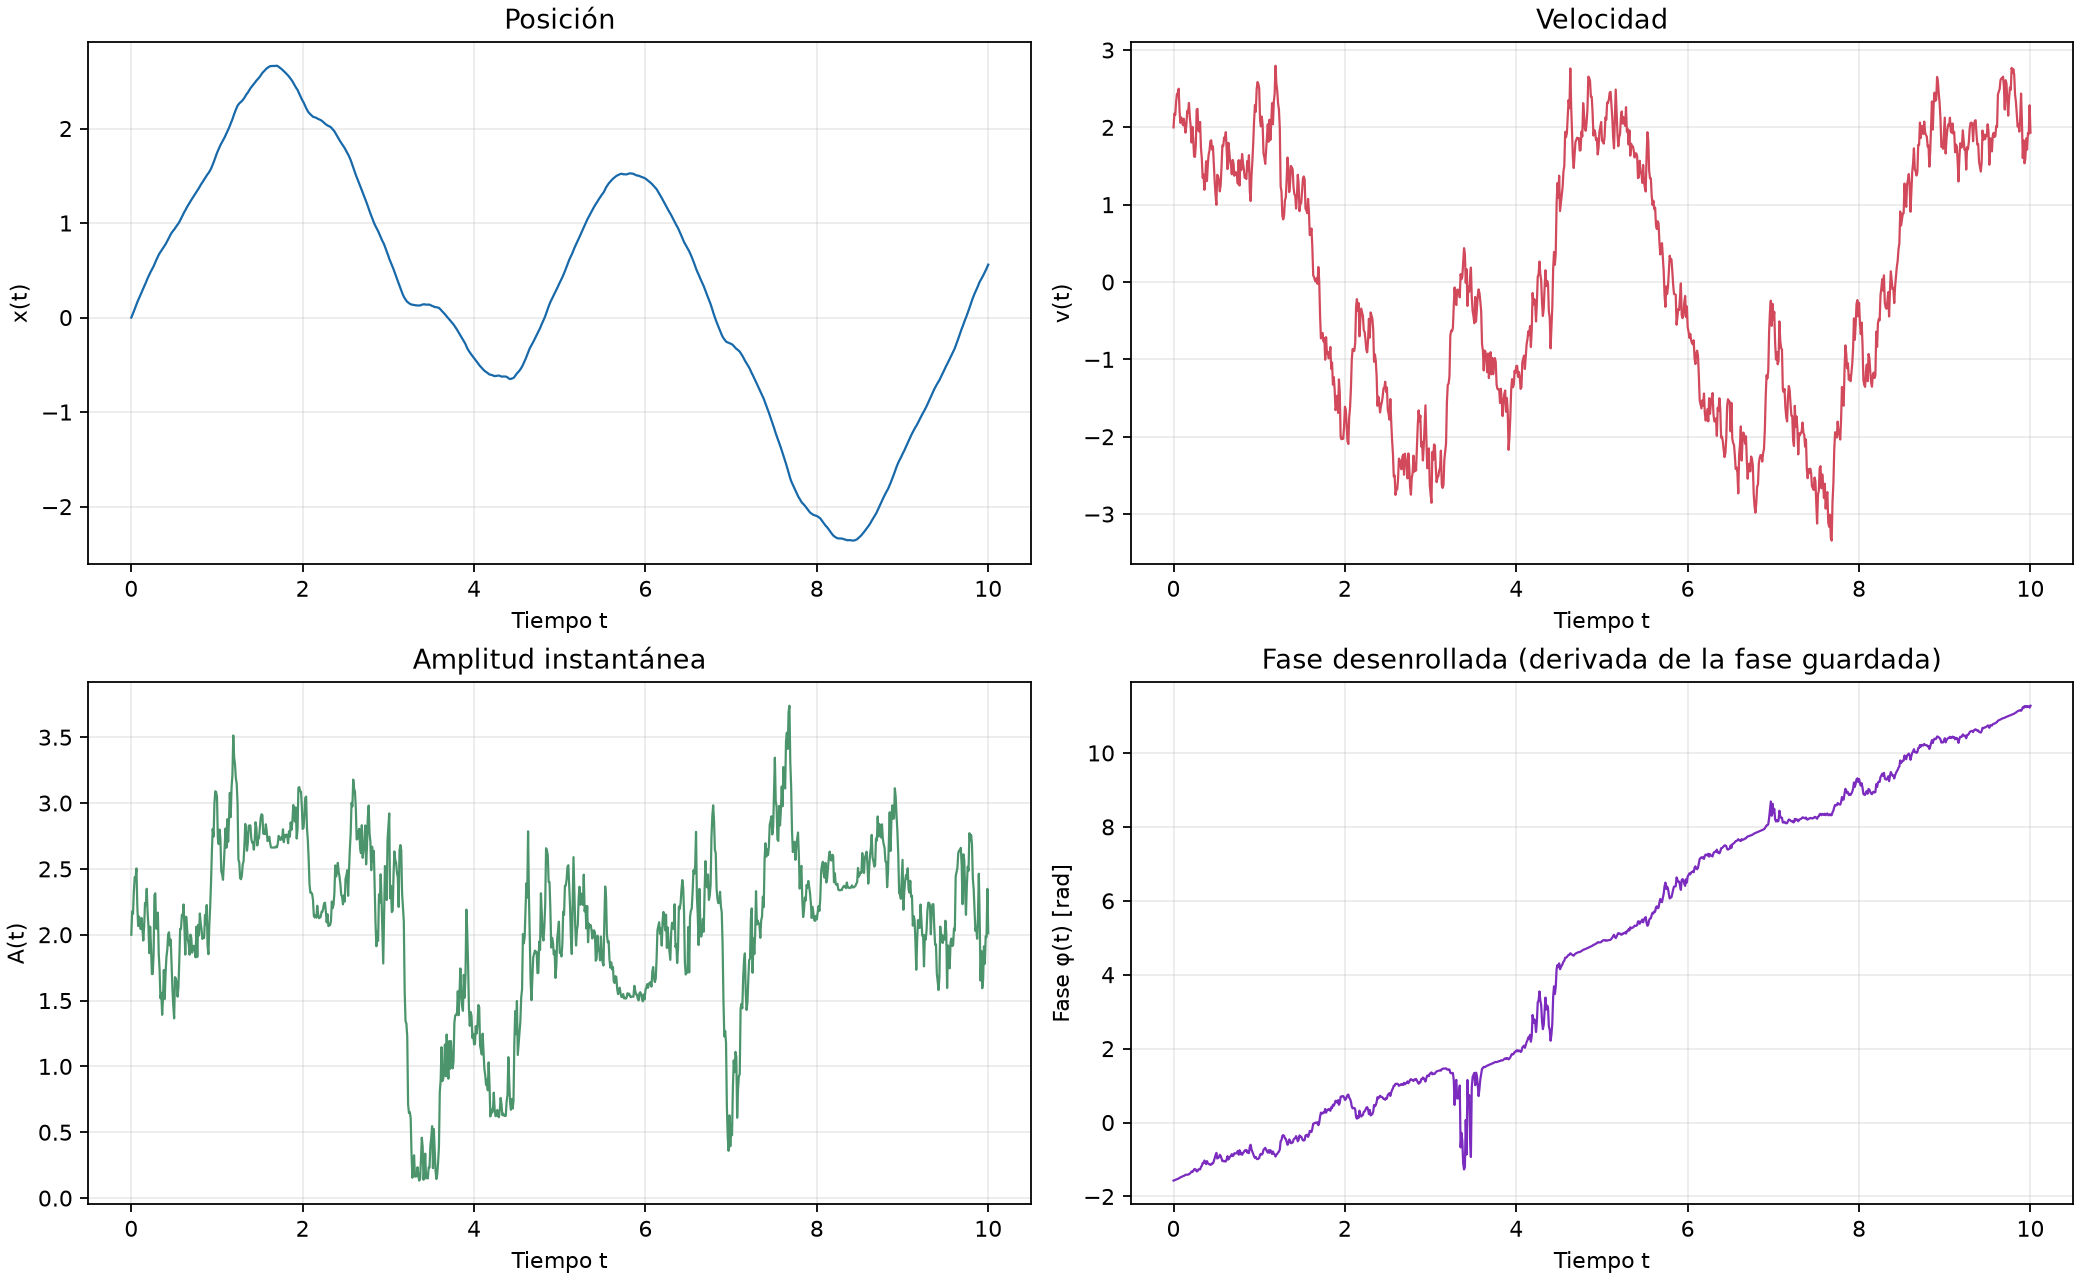
\includegraphics[width=0.9\linewidth]{Fig.png}
        \caption{Gráficas del oscilador de posición, velocidad, amplitud y fase del oscilador de Rayleight}
    \end{figure}

    Tras la realización de múltiples experimentos variando condiciones iniciales y distintos pesos para el ruido estocástico como se puede ver en la figura 2.

    \begin{figure}[H]
        \centering
        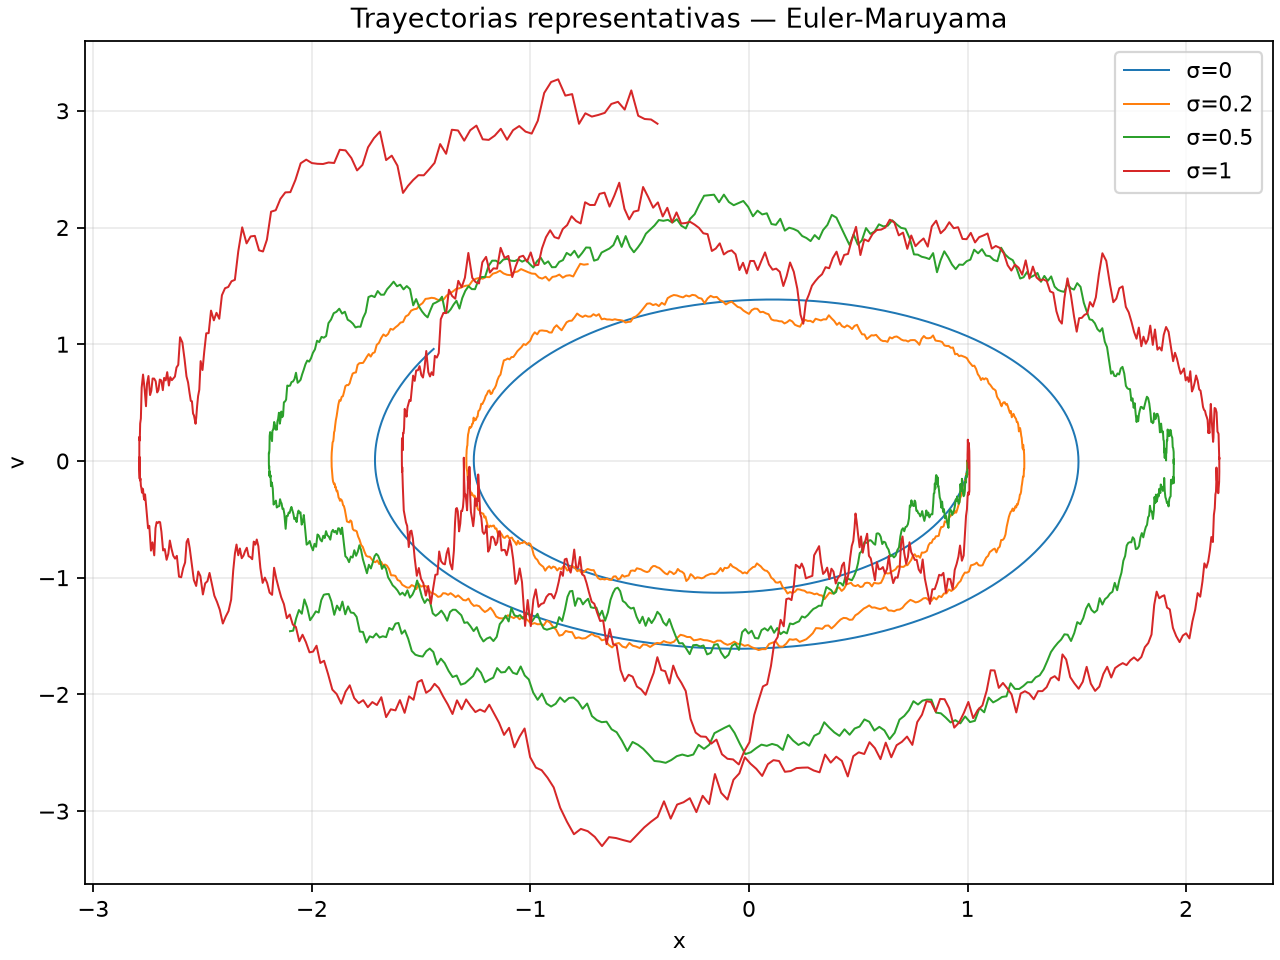
\includegraphics[width=0.9\linewidth]{espacioFase.png}
        \caption{Gráfica del espacio de fase el oscilador de Rayleigh con ruido estocástico mediante el método de Euler-Maruyama para distintos $\sigma$.}
    \end{figure}

    Se logró evidenciar que conforme aumento el peso del ruido ---$\sigma$---, el ciclo límite presenta las fluctuaciones que se esperaban teóricamente pero se mantienen constantes dada la utilización de una semilla fija para los experimentos.

\end{multicols}

%%%%%%%%%%%%%%%%%%%%%%%%%%%%%%%%%


\section*{Referencias}

\begin{enumerate}
    
    \item \href{https://es.scribd.com/document/140663057/Landau-and-Lifshitz-Course-of-Theoretical-Physics-Vol-10-Physical-Kinetics}{Landau \& Lifshitz -- Vol. 10 -- Physical-Kinetics.}

    \item \href{https://pt.scribd.com/document/375435049/C-W-Gardiner-Handbook-of-Stochastic-Methods-B-ok-org}{C.W. Gardiner - Handbook of Stochastic Methods for Physics, Chemistry and the Natural Sciences}
    
\end{enumerate}

\end{document}
